\documentclass[11pt]{article}

\usepackage[margin=0.75in]{geometry}
\usepackage[T1]{fontenc}
\usepackage[utf8]{inputenc}
\usepackage{lmodern}
\usepackage{amsmath,amssymb}
\usepackage{booktabs}
\usepackage{graphicx}
\usepackage{xcolor}
\usepackage{hyperref}
\usepackage{float}
\usepackage{caption}
\usepackage{enumitem}

\hypersetup{
  colorlinks=true,
  linkcolor=blue!50!black,
  urlcolor=blue!50!black
}

\setlist[itemize]{leftmargin=1.2em,itemsep=0.25em}
\setlength{\parskip}{0.45em}
\setlength{\parindent}{0pt}

\title{Stage III Topology Pass on Frozen \texttt{dataset\_iter035}}
\author{Run ID: \texttt{topology\_pass\_dataset\_iter035\_v1}}
\date{June 20, 2026}

\begin{document}
\maketitle

\begin{abstract}
This report documents an offline topology classification and compute-cost audit
on the frozen thermodynamic active-learning dataset \texttt{dataset\_iter035}.
The original thermodynamic labels, exact-oracle outputs, acquisition logic,
and active-learning loop were not modified.  The goal is to compute Pfaffian
$\mathbb{Z}_2$ diagnostics and a full-Brillouin-zone bulk quasiparticle gap on
existing superconducting exact points, then identify coverage gaps and
candidate seeds for a future topology-aware acquisition stage.  The sparse
topology scatter and Delaunay edges reported here are diagnostic seeds only;
they are not final topological phase boundaries.
\end{abstract}

\section{Scope and Inputs}

The frozen thermodynamic dataset contains 7434 exact points:
\begin{itemize}
  \item normal: 1867,
  \item uniform-SC: 715,
  \item FFLO: 4852.
\end{itemize}
Only the existing superconducting points were passed through the topology
oracle.  Normal points are retained in the derived output with
\texttt{topology\_label = not\_applicable}.  No new $\Delta$-$q$ exact search
or active-learning iteration was run.

The main generated artifacts are:
\begin{itemize}
  \item \texttt{tables/dataset\_iter035\_topology\_ground\_v1.csv},
  \item \texttt{tables/dataset\_iter035\_topology\_ground\_v1.npz},
  \item \texttt{topology\_pass\_summary.json},
  \item \texttt{topology\_benchmark\_report.json},
  \item \texttt{topology\_validation\_report.md},
  \item this LaTeX report and its compiled PDF.
\end{itemize}
Parquet output was requested by the Stage III plan but was not written in this
local environment because neither \texttt{pyarrow} nor \texttt{fastparquet} is
installed.  The CSV and NPZ outputs contain the full derived dataset.

\section{BdG and Pfaffian Convention}

The topology pass reuses the project BdG Hamiltonian builder for the
full-Brillouin-zone bulk gap.  The analytic Pfaffian convention was not chosen
by inspection alone; it was cross-checked against a numerical Pfaffian built
from the project BdG Hamiltonian in the current Nambu/Majorana convention.

The verified convention is
\begin{align}
P_0 &=
\left(\mu - t\cos\frac{q}{2}\right)^2 + \Delta^2
- \alpha_y^2\sin^2\frac{q}{2}
- \left(J_A\cos\frac{q}{2}+\alpha_z\sin\frac{q}{2}\right)^2,\\
P_\pi &=
\left(\mu + t\cos\frac{q}{2}\right)^2 + \Delta^2
- \alpha_y^2\sin^2\frac{q}{2}
- \left(J_A\cos\frac{q}{2}+\alpha_z\sin\frac{q}{2}\right)^2.
\end{align}
For gapped and reliable superconducting points,
\[
P_0P_\pi < 0 \Rightarrow \mathbb{Z}_2 = 1,\qquad
P_0P_\pi > 0 \Rightarrow \mathbb{Z}_2 = 0.
\]
The dimensionless Pfaffian margin is
\[
m_{\mathrm{Pf}} =
\frac{\min(|P_0|,|P_\pi|)}{E_{\mathrm{scale}}^2},
\]
where $E_{\mathrm{scale}}$ is constructed from the model energy scales rather
than set by an arbitrary fixed unit.

The analytic and numerical Pfaffian product signs agreed on all 104
non-boundary validation points.  This check is a gate: the full pass should not
be interpreted if this product-sign agreement fails.

\section{Bulk-Gap Oracle and Resource Decision}

The bulk quasiparticle gap is computed as
\[
E_g = \min_{k,n}|E_n(k)|,
\]
over one full Brillouin zone.  The implementation uses float64/complex128,
chunked batched eigensolves, and does not store full spectra for all points.
The final coarse grid used $N_k=2048$.  For small-gap, small-Pfaffian-margin,
and 5\% random-control points, the pass performed both $N_k$ doubling and
bounded local minimization around the coarse minimum.

The 256-point pilot benchmark selected the GPU backend by measurement, not by
assumption.  CPU/GPU agreement at $N_k=2048$ had maximum absolute bulk-gap
difference $7.77\times10^{-16}$.  The full bulk-gap scan recorded in the
summary took 5.342 seconds on the RTX 4090 backend; the complete script,
including local $k$ refinement and report outputs, ran in roughly 70 seconds.

\section{Topology Classification Results}

\begin{table}[H]
\centering
\caption{Topology label counts by thermodynamic phase.}
\begin{tabular}{llr}
\toprule
Thermodynamic phase & Topology label & Count\\
\midrule
uniform-SC & trivial & 715\\
uniform-SC & topological & 0\\
uniform-SC & gapless\_SC & 0\\
uniform-SC & topology\_unresolved & 0\\
FFLO & trivial & 3127\\
FFLO & topological & 1515\\
FFLO & gapless\_SC & 195\\
FFLO & topology\_unresolved & 15\\
\bottomrule
\end{tabular}
\end{table}

Across all 5567 superconducting points, 5357 points have trusted topology
labels under the current bulk-gap and exact-label reliability rules.  The 195
\texttt{gapless\_SC} points are points where the local $k$-refined bulk-gap
oracle resolved the spectrum as gapless under the current tolerance.  The 15
\texttt{topology\_unresolved} points remain numerical-reliability states and
must not be interpreted as a physical phase.

\section{Coverage and Boundary-Seed Diagnostics}

Trusted gapped FFLO points were used to construct a Delaunay diagnostic graph
in normalized $(k_BT,J_A)$ space.  This graph is used only to identify
candidate topology-boundary seeds and sampling holes.

\begin{table}[H]
\centering
\caption{Topology-boundary seed and coverage diagnostics.}
\begin{tabular}{lr}
\toprule
Diagnostic & Value\\
\midrule
Trusted FFLO gapped points & 4642\\
Delaunay edges & 13575\\
Delaunay triangles & 8934\\
$\mathbb{Z}_2$-change candidate edges & 182\\
$P_0$ sign-change candidate edges & 182\\
$P_\pi$ sign-change candidate edges & 0\\
Large circumradius coverage-hole triangles & 447\\
Nearest-neighbor p95 distance, normalized & 0.0117625\\
Nearest-neighbor max distance, normalized & 0.0549629\\
\bottomrule
\end{tabular}
\end{table}

All candidate $\mathbb{Z}_2$-change edges are associated with $P_0$ sign
changes in this diagnostic graph.  This supports a topology-aware follow-up,
but it does not by itself define a final contour.

\begin{figure}[H]
\centering
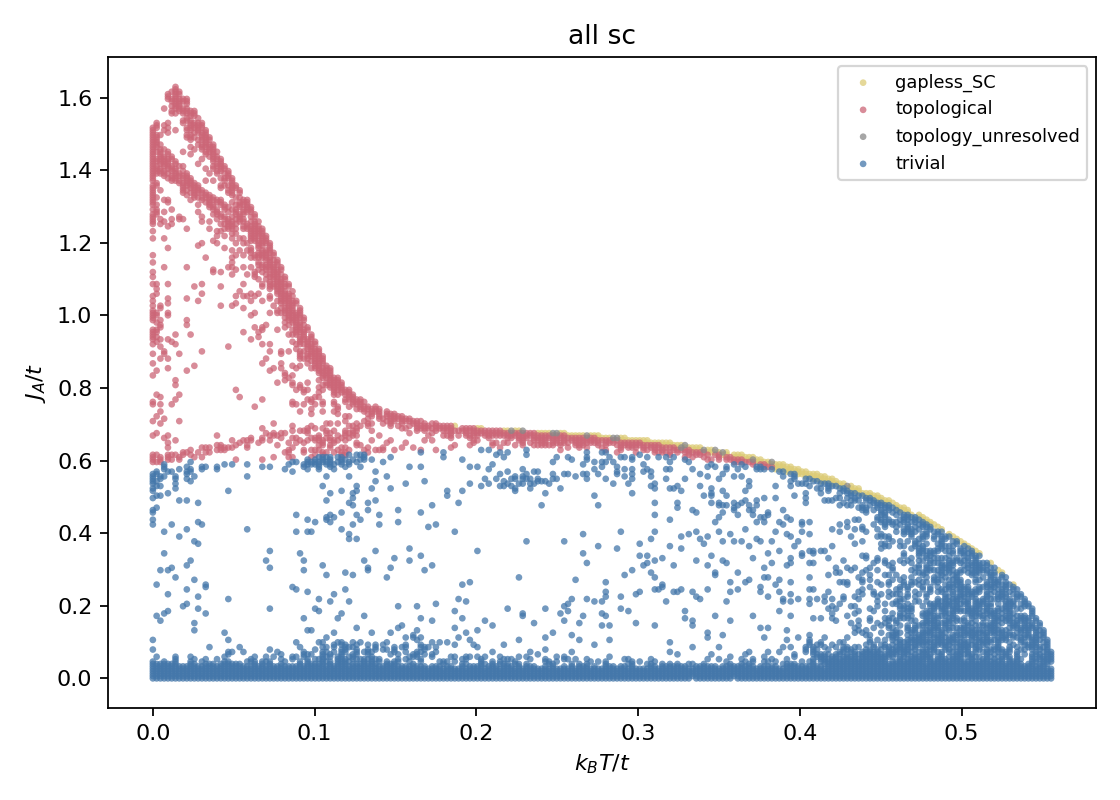
\includegraphics[width=0.86\linewidth]{figures/topology_scatter_all_sc.png}
\caption{Offline topology labels for all superconducting points.  This is a
scatter diagnostic, not an interpolated final topological phase boundary.}
\end{figure}

\begin{figure}[H]
\centering
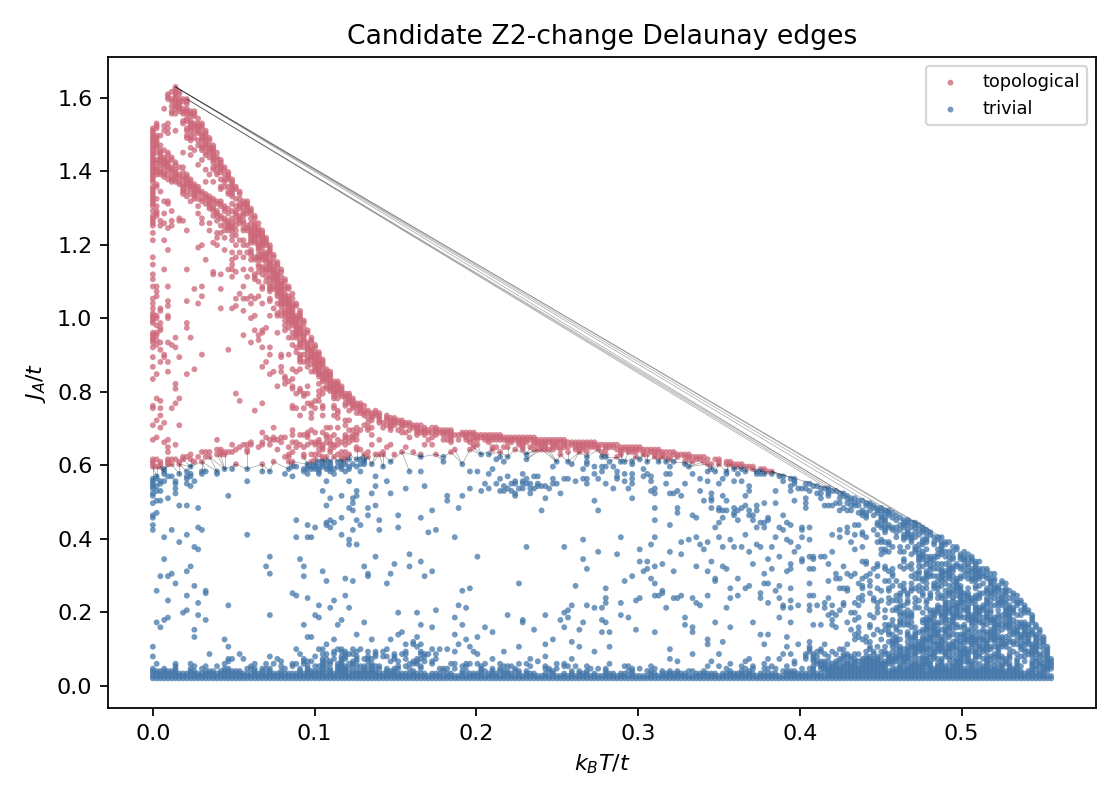
\includegraphics[width=0.86\linewidth]{figures/topology_boundary_candidate_edges.png}
\caption{Candidate $\mathbb{Z}_2$-change Delaunay edges among trusted gapped
FFLO points.  These edges are seeds for targeted topology refinement.}
\end{figure}

\begin{figure}[H]
\centering
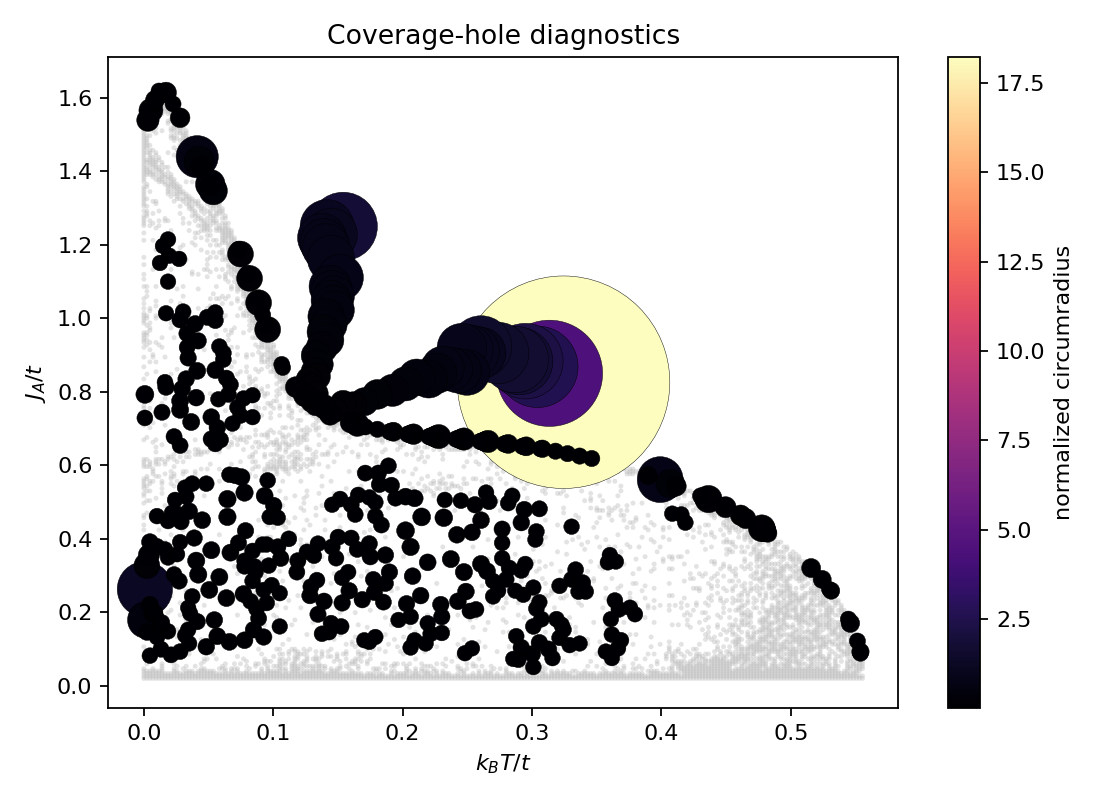
\includegraphics[width=0.86\linewidth]{figures/topology_coverage_holes.png}
\caption{Large-circumradius Delaunay triangles used as sampling coverage-hole
diagnostics.}
\end{figure}

\begin{figure}[H]
\centering
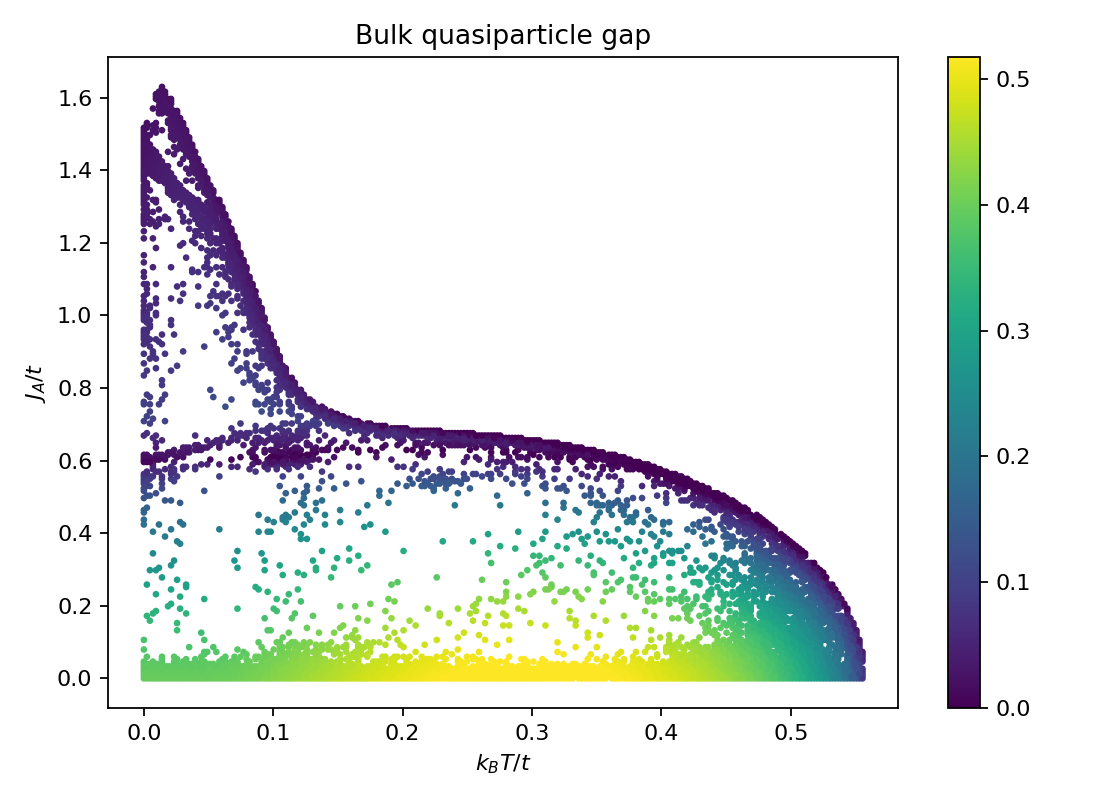
\includegraphics[width=0.86\linewidth]{figures/bulk_gap_scatter.png}
\caption{Full-Brillouin-zone bulk quasiparticle gap over superconducting
points.}
\end{figure}

\section{Caveats}

\begin{itemize}
  \item Do not modify or reinterpret the original normal / uniform-SC / FFLO
  labels from this topology pass.
  \item Do not call sparse Delaunay edges final topology contours.
  \item Do not treat \texttt{topology\_unresolved} as a gapless phase.
  \item Do not use the Pfaffian sign without the full bulk-gap status.
  \item Hard-risk or provisional exact points are diagnostics only unless
  separately audited.
  \item The current result is single-dataset and single-pass; it is not yet a
  multi-seed benchmark.
\end{itemize}

\section{Decision}

The result falls under Case B of the Stage III plan:

\begin{quote}
Trusted topological and trivial FFLO points exist, but inherited sampling is
not dense enough near candidate topology boundaries to claim a final
topological contour.
\end{quote}

The recommended next calculation is a topology-aware acquisition/refinement
pilot that targets:
\begin{itemize}
  \item small Pfaffian margin,
  \item small bulk gap,
  \item candidate $\mathbb{Z}_2$-change Delaunay edges,
  \item large coverage-hole regions.
\end{itemize}
This should not restart the thermodynamic active-learning loop.  It should
operate as a topology-focused follow-up on the frozen thermodynamic phase map.

\end{document}
